% Divide and Conquer Part 1 -- Metropolis beamer slides
% Compile: pdflatex divide-and-conquer-1.tex (x2)
\documentclass[10pt,aspectratio=169]{beamer}

\usetheme{metropolis}
\metroset{block=fill, numbering=fraction, progressbar=frametitle}

\usepackage[T1]{fontenc}
\usepackage{amsmath, amssymb}
\usepackage{listings}
\usepackage{booktabs}
\usepackage{tikz}
\usepackage{pgfplots}
\pgfplotsset{compat=1.18}
\usetikzlibrary{arrows.meta, positioning, decorations.pathreplacing, calc, trees}

% ---- colors -------------------------------------------------------------
\definecolor{mLightBlue}{HTML}{4C72B0}
\definecolor{mGreen}{HTML}{55A868}
\definecolor{mRed}{HTML}{C44E52}
\definecolor{mGray}{HTML}{BFBFBF}
\setbeamercolor{alerted text}{fg=mRed}

% ---- code style ---------------------------------------------------------
\lstdefinestyle{jl}{
  basicstyle=\ttfamily\footnotesize,
  keywordstyle=\color{mRed}\bfseries,
  commentstyle=\color{mGreen}\itshape,
  numberstyle=\tiny\color{mGray},
  showstringspaces=false,
  breaklines=true,
  columns=fullflexible,
  morekeywords={function,for,in,if,else,elseif,end,return,length,while,view}
}
\lstset{style=jl}

% ---- helpers ------------------------------------------------------------
% \cells{list}{index to highlight}{fill for highlight}
\newcommand{\cells}[3]{%
  \begin{tikzpicture}[scale=0.8, every node/.style={transform shape}]
    \foreach \v [count=\i from 0] in {#1} {
      \pgfmathtruncatemacro{\hl}{#2}
      \ifnum\i=\hl \def\fillc{#3}\else\def\fillc{black!5}\fi
      \node[draw, minimum size=7mm, fill=\fillc] at (\i*0.75,0) {\small \v};
    }
  \end{tikzpicture}%
}

% ---- merge animation ----------------------------------------------------
% \mergestep{ja}{jb}{C contents, "." = empty slot}{caption}
% ja, jb are 0-indexed; a value > 2 means that array is exhausted.
\newcommand{\mergestep}[4]{%
  \begin{center}
  \begin{tikzpicture}[scale=0.85, every node/.style={transform shape},
      cell/.style={draw, minimum size=7mm},
      ptr/.style={-{Stealth}, very thick}]
    % ---- A
    \node[left] at (-0.5,1.6) {\small $A$:};
    \foreach \v [count=\i from 0] in {1,4,9} {
      \ifnum\i<#1 \def\fillc{black!8}\else\def\fillc{mLightBlue!30}\fi
      \node[cell, fill=\fillc] at (\i*0.85,1.6) {\small \v};
    }
    % ---- B
    \node[left] at (-0.5,0.2) {\small $B$:};
    \foreach \v [count=\i from 0] in {2,3,7} {
      \ifnum\i<#2 \def\fillc{black!8}\else\def\fillc{mGreen!30}\fi
      \node[cell, fill=\fillc] at (\i*0.85,0.2) {\small \v};
    }
    % ---- pointers
    \ifnum#1>2
      \node[mGray] at (2.55,2.6) {\small $j_a$: done};
    \else
      \draw[ptr, mLightBlue] (#1*0.85,2.45) -- (#1*0.85,2.02);
      \node[mLightBlue] at (#1*0.85,2.78) {\small $j_a$};
    \fi
    \ifnum#2>2
      \node[mGray] at (2.55,-0.85) {\small $j_b$: done};
    \else
      \draw[ptr, mGreen] (#2*0.85,-0.68) -- (#2*0.85,-0.25);
      \node[mGreen] at (#2*0.85,-1.0) {\small $j_b$};
    \fi
    % ---- C
    \node[left] at (-0.5,-2.2) {\small $C$:};
    \foreach \v [count=\i from 0] in {#3} {
      \edef\tmp{\v}\def\blank{.}
      \ifx\tmp\blank
        \node[cell, draw=mGray, fill=white] at (\i*0.85,-2.2) {};
      \else
        \node[cell, fill=black!8] at (\i*0.85,-2.2) {\small \v};
      \fi
    }
  \end{tikzpicture}
  \end{center}
  \begin{center}#4\end{center}%
}

% ---- title --------------------------------------------------------------
\title{Divide and Conquer, Part 1}
\subtitle{Tiling Puzzle, Binary Search, Merge Sort, Solving Recurrences}
\date{}
\author{}

\begin{document}

\maketitle

% =========================================================================
\begin{frame}{The Paradigm}
  \begin{itemize}
    \item \alert{Divide} a problem of size $n$ into smaller sub-problems.
    \item \alert{Conquer} them recursively.
    \item \alert{Combine} their solutions into a solution for the original.
    \item Small $n$ is solved directly: the \alert{base case}.
  \end{itemize}

  \bigskip
  \begin{center}
  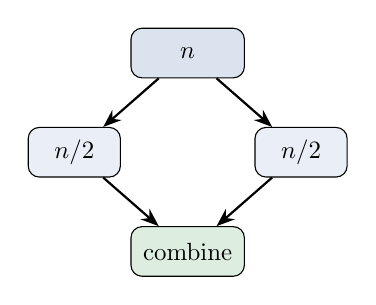
\begin{tikzpicture}[scale=0.9, every node/.style={transform shape}]
    \node[draw, rounded corners, fill=mLightBlue!20, minimum width=16mm, minimum height=7mm] (p) at (0,1.4) {$n$};
    \node[draw, rounded corners, fill=mLightBlue!12, minimum width=13mm, minimum height=7mm] (a) at (-1.6,0) {$n/2$};
    \node[draw, rounded corners, fill=mLightBlue!12, minimum width=13mm, minimum height=7mm] (b) at (1.6,0) {$n/2$};
    \node[draw, rounded corners, fill=mGreen!20, minimum width=16mm, minimum height=7mm] (c) at (0,-1.4) {combine};
    \draw[-{Stealth}, thick] (p) -- (a);
    \draw[-{Stealth}, thick] (p) -- (b);
    \draw[-{Stealth}, thick] (a) -- (c);
    \draw[-{Stealth}, thick] (b) -- (c);
  \end{tikzpicture}
  \end{center}
\end{frame}

% =========================================================================
\section{Tiling Puzzle}

\begin{frame}{The Puzzle}
  A $2^n \times 2^n$ board has \alert{one missing square}.
  Tile the rest with L-shaped trominoes, with no overlaps and nothing off the board.

  \bigskip
  \begin{center}
  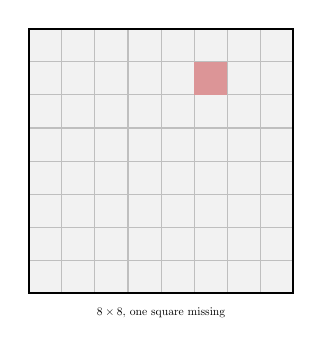
\begin{tikzpicture}[scale=0.42, every node/.style={transform shape}]
    \foreach \x in {0,...,7} \foreach \y in {0,...,7} {
      \fill[black!5] (\x,\y) rectangle ++(1,1);
      \draw[mGray] (\x,\y) rectangle ++(1,1);
    }
    \fill[mRed!60] (5,6) rectangle ++(1,1);
    \draw[thick] (0,0) rectangle (8,8);
    \node[below] at (4,-0.3) {\normalsize $8 \times 8$, one square missing};
  \end{tikzpicture}
  \end{center}
\end{frame}

\begin{frame}{Base Case: $2 \times 2$}
  Trivial: orient the single tromino away from the missing square.

  \bigskip
  \begin{center}
  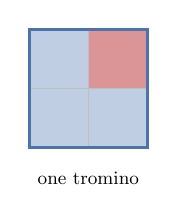
\begin{tikzpicture}[scale=0.75, every node/.style={transform shape}]
    \foreach \x in {0,1} \foreach \y in {0,1} {
      \fill[mLightBlue!35] (\x,\y) rectangle ++(1,1);
      \draw[mGray] (\x,\y) rectangle ++(1,1);
    }
    \fill[mRed!60] (1,1) rectangle ++(1,1);
    \draw[mGray] (1,1) rectangle ++(1,1);
    \draw[very thick, mLightBlue] (0,0) rectangle (2,2);
    \node[below] at (1,-0.3) {\small one tromino};
  \end{tikzpicture}
  \end{center}
\end{frame}

\begin{frame}{Exercise}
  \begin{center}
    How do you reduce the $4 \times 4$ case to the $2 \times 2$ case?
  \end{center}

  \bigskip
  \begin{center}
  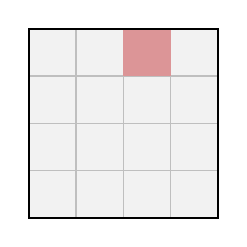
\begin{tikzpicture}[scale=0.6, every node/.style={transform shape}]
    \foreach \x in {0,...,3} \foreach \y in {0,...,3} {
      \fill[black!5] (\x,\y) rectangle ++(1,1);
      \draw[mGray] (\x,\y) rectangle ++(1,1);
    }
    \fill[mRed!60] (2,3) rectangle ++(1,1);
    \draw[thick] (0,0) rectangle (4,4);
  \end{tikzpicture}
  \end{center}

  \bigskip
  \begin{center}
    \small Pause and think before the next slide.
  \end{center}
\end{frame}

\begin{frame}{Solution}
  Split into four quadrants. One already has the missing square.
  Place \alert{one tromino in the center} covering the other three.

  \bigskip
  \begin{center}
  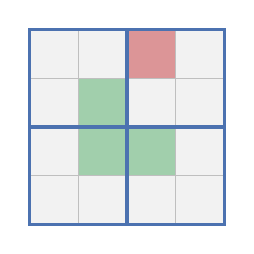
\begin{tikzpicture}[scale=0.62, every node/.style={transform shape}]
    \foreach \x in {0,...,3} \foreach \y in {0,...,3} {
      \fill[black!5] (\x,\y) rectangle ++(1,1);
      \draw[mGray] (\x,\y) rectangle ++(1,1);
    }
    % centre tromino: covers the three quadrants without the hole
    \fill[mGreen!55] (1,1) rectangle ++(1,1);
    \fill[mGreen!55] (2,1) rectangle ++(1,1);
    \fill[mGreen!55] (1,2) rectangle ++(1,1);
    \foreach \x in {1,2} \foreach \y in {1,2} \draw[mGray] (\x,\y) rectangle ++(1,1);
    \fill[mRed!60] (2,3) rectangle ++(1,1);
    \draw[mGray] (2,3) rectangle ++(1,1);
    % quadrant borders
    \draw[very thick, mLightBlue] (0,0) rectangle (2,2);
    \draw[very thick, mLightBlue] (2,0) rectangle (4,2);
    \draw[very thick, mLightBlue] (0,2) rectangle (2,4);
    \draw[very thick, mLightBlue] (2,2) rectangle (4,4);
  \end{tikzpicture}
  \end{center}

  \bigskip
  Now every quadrant is a $2 \times 2$ board with one square missing, which is the base case.
\end{frame}

\begin{frame}{The General Recursion}
  The same move works at every scale:

  \bigskip
  \begin{itemize}
    \item Split the $2^n \times 2^n$ board into four $2^{n-1} \times 2^{n-1}$ quadrants.
    \item One quadrant holds the missing square.
    \item Drop one tromino in the center to punch a hole in each of the other three.
    \item Recurse on all four.
  \end{itemize}

  \bigskip
  \begin{center}
    Every board of this shape can be tiled.
  \end{center}
\end{frame}

% =========================================================================
\section{Binary Search}

\begin{frame}{Binary Search}
  \textbf{Input:} a \alert{sorted} array $A[1 \ldots n]$ and a value $x$.\\
  \textbf{Output:} whether $x$ occurs in $A$.

  \bigskip
  Look at the middle $m = \lfloor n/2 \rfloor$. If $x \le A[m]$, search $A[1 \ldots m]$; otherwise search $A[m+1 \ldots n]$.

  \bigskip
  \begin{center}
  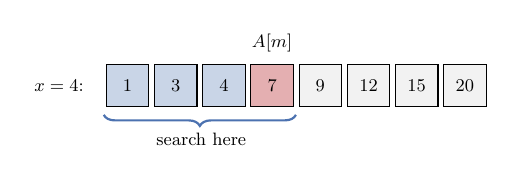
\begin{tikzpicture}[scale=0.72, every node/.style={transform shape}]
    \foreach \v [count=\i from 0] in {1,3,4,7,9,12,15,20} {
      \ifnum\i<4 \def\fillc{mLightBlue!30}\else\def\fillc{black!5}\fi
      \ifnum\i=3 \def\fillc{mRed!45}\fi
      \node[draw, minimum size=7.5mm, fill=\fillc] at (\i*0.85,0) {\small \v};
    }
    \node[left] at (-0.65,0) {\small $x = 4$:};
    \draw[decorate, decoration={brace, amplitude=4pt}, mLightBlue, thick]
      (2.97,-0.52) -- (-0.42,-0.52);
    \node[below] at (1.3,-0.72) {\small search here};
    \node[above] at (2.55,0.46) {\small $A[m]$};
  \end{tikzpicture}
  \end{center}

  \bigskip
  \begin{center}
    Each step \alert{halves} the search range.
  \end{center}
\end{frame}

\begin{frame}[fragile]{Recursive Version}
  \begin{lstlisting}
function binary_search(A, x, i, j)
    # Check if x is in A[i:j].
    # Return the index of x if found, otherwise nothing
    if i == j
        # Base case
        A[i] == x ? return i : return nothing
    else
        m = floor(Int, (i + j) / 2)
        if x <= A[m]
            return binary_search(A, x, i, m)
        else
            return binary_search(A, x, m + 1, j)
        end
    end
end
  \end{lstlisting}
\end{frame}

\begin{frame}{Running Time}
  \begin{itemize}
    \item The range starts at $n$ and halves each level.
    \item Each level does $O(1)$ non-recursive work.
    \item At level $i$ the range is $n/2^i$; setting $n/2^i = 1$ gives $i = \log_2 n$.
  \end{itemize}

  \bigskip
  \begin{center}
  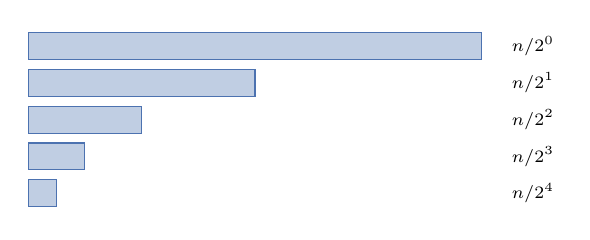
\begin{tikzpicture}[scale=0.9, every node/.style={transform shape}]
    \foreach \w [count=\i from 0] in {6.4, 3.2, 1.6, 0.8, 0.4} {
      \fill[mLightBlue!35, draw=mLightBlue] (0,-\i*0.52) rectangle ++(\w,0.38);
      \node[right] at (6.7,-\i*0.52+0.19) {\scriptsize $n/2^{\i}$};
    }
  \end{tikzpicture}
  \end{center}

  \bigskip
  \begin{alertblock}{Total}
    $O(\log n) \times O(1) = O(\log n)$
  \end{alertblock}
\end{frame}

\begin{frame}[fragile]{Iterative Version}
  Often written iteratively, since it is simpler.

  \begin{lstlisting}
# Return the index of x in A if found, otherwise nothing
function binary_search(A, x)
    i, j = 1, length(A)
    while i < j
        m = floor(Int, (i + j) / 2)
        if x <= A[m]
            j = m
        else
            i = m + 1
        end
    end
    return (i <= length(A) && A[i] == x) ? i : -1
end
  \end{lstlisting}
\end{frame}

% =========================================================================
\section{Merge Sort}

\begin{frame}{Merging Two Sorted Arrays}
  Repeatedly take the smaller of the two front elements.

  \bigskip
  \begin{center}
  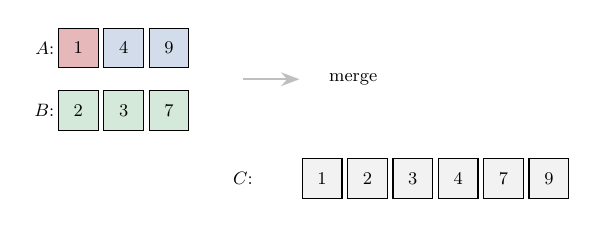
\begin{tikzpicture}[scale=0.72, every node/.style={transform shape}]
    \node[left] at (-0.3,1.2) {\small $A$:};
    \foreach \v [count=\i from 0] in {1,4,9} {
      \ifnum\i=0 \def\fillc{mRed!40}\else\def\fillc{mLightBlue!25}\fi
      \node[draw, minimum size=7mm, fill=\fillc] at (\i*0.8,1.2) {\small \v};
    }
    \node[left] at (-0.3,0.1) {\small $B$:};
    \foreach \v [count=\i from 0] in {2,3,7} {
      \node[draw, minimum size=7mm, fill=mGreen!25] at (\i*0.8,0.1) {\small \v};
    }
    \draw[-{Stealth}, thick, mGray] (2.9,0.65) -- (3.9,0.65);
    \node[left] at (3.2,-1.1) {\small $C$:};
    \foreach \v [count=\i from 0] in {1,2,3,4,7,9} {
      \node[draw, minimum size=7mm, fill=black!5] at (4.3+\i*0.8,-1.1) {\small \v};
    }
    \node[right] at (4.3,0.65) {\small merge};
  \end{tikzpicture}
  \end{center}

  
\end{frame}

% ---------------------------------------------------------------- animation
\begin{frame}{Merging Step by Step}
  \mergestep{0}{0}{.,.,.,.,.,.}{Compare $1$ and $2$. \quad Take \alert{$1$} from $A$.}
\end{frame}

\begin{frame}{Merging Step by Step}
  \mergestep{1}{0}{1,.,.,.,.,.}{Compare $4$ and $2$. \quad Take \alert{$2$} from $B$.}
\end{frame}

\begin{frame}{Merging Step by Step}
  \mergestep{1}{1}{1,2,.,.,.,.}{Compare $4$ and $3$. \quad Take \alert{$3$} from $B$.}
\end{frame}

\begin{frame}{Merging Step by Step}
  \mergestep{1}{2}{1,2,3,.,.,.}{Compare $4$ and $7$. \quad Take \alert{$4$} from $A$.}
\end{frame}

\begin{frame}{Merging Step by Step}
  \mergestep{2}{2}{1,2,3,4,.,.}{Compare $9$ and $7$. \quad Take \alert{$7$} from $B$.}
\end{frame}

\begin{frame}{Merging Step by Step}
  \mergestep{2}{3}{1,2,3,4,7,.}{$B$ is exhausted. \quad Copy the rest of $A$.}
\end{frame}

\begin{frame}{Merging Step by Step}
  \mergestep{3}{3}{1,2,3,4,7,9}{Done.}

  \bigskip
  \begin{center}
    Each element is touched once, so merging costs $O(n + m)$.
  \end{center}
\end{frame}

\begin{frame}[fragile]{The Merge Procedure}
  \begin{lstlisting}
function merge(A, B)
    n, m = length(A), length(B)
    C = Vector{eltype(A)}(undef, n + m)
    ja = jb = j = 1

    while ja <= n && jb <= m
        if A[ja] <= B[jb]
            C[j] = A[ja]; ja += 1
        else
            C[j] = B[jb]; jb += 1
        end
        j += 1
    end

    while ja <= n;  C[j] = A[ja]; ja += 1; j += 1; end
    while jb <= m;  C[j] = B[jb]; jb += 1; j += 1; end
    return C
end
  \end{lstlisting}

  
\end{frame}

\begin{frame}[fragile]{Merge Sort}
  Sort each half recursively, then merge.

  \begin{lstlisting}
function merge_sort(A)
    n = length(A)
    if n <= 1
        return A
    else
        mid = n div 2
        L = @view A[1:mid]
        R = @view A[mid+1:end]

        sorted_L = merge_sort(L)
        sorted_R = merge_sort(R)

        return merge(sorted_L, sorted_R)
    end
end
  \end{lstlisting}
\end{frame}

\begin{frame}{Merge Sort: Recurrence}
  Correctness is clear: after the recursive calls $L$ and $R$ are sorted, and merging preserves order.

  \bigskip
  Each level does $O(n)$ non-recursive work and makes two calls of half the size:

  \begin{alertblock}{}
    \[
      T(n) = 2\,T(n/2) + O(n)
    \]
  \end{alertblock}

  \bigskip
  \begin{center}
    We will show $T(n) = O(n \log n)$, and in fact $\Theta(n \log n)$.\\
    \smallskip
    \small Compare with selection sort's $O(n^2)$.
  \end{center}
\end{frame}

% =========================================================================
\section{Solving Recurrences}

\begin{frame}{Recursion Trees}
  Draw one node per call. The running time is the \alert{total non-recursive work} in the tree.

  \bigskip
  Three things can happen as you go down:

  \begin{itemize}
    \item Work per level stays the \alert{same}: multiply by the number of levels.
    \item Work per level \alert{shrinks} geometrically: the root dominates.
    \item Work per level \alert{grows} geometrically: the leaves dominate.
  \end{itemize}
\end{frame}

% ---------------------------------------------------------------- case 1
\begin{frame}{Case 1: Equal Work Per Level}
  $T(n) = 2T(n/2) + cn$ \quad (merge sort)

  \begin{center}
  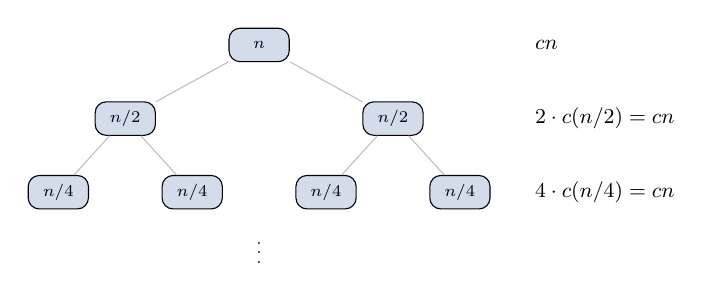
\begin{tikzpicture}[scale=0.85, every node/.style={transform shape},
      lv/.style={draw, rounded corners, fill=mLightBlue!25, minimum width=9mm, minimum height=5mm, inner sep=1pt}]
    \node[lv] (a) at (0,0) {\scriptsize $n$};
    \node[lv] (b1) at (-2,-1.1) {\scriptsize $n/2$};
    \node[lv] (b2) at (2,-1.1) {\scriptsize $n/2$};
    \node[lv] (c1) at (-3,-2.2) {\scriptsize $n/4$};
    \node[lv] (c2) at (-1,-2.2) {\scriptsize $n/4$};
    \node[lv] (c3) at (1,-2.2) {\scriptsize $n/4$};
    \node[lv] (c4) at (3,-2.2) {\scriptsize $n/4$};
    \draw[mGray] (a) -- (b1); \draw[mGray] (a) -- (b2);
    \draw[mGray] (b1) -- (c1); \draw[mGray] (b1) -- (c2);
    \draw[mGray] (b2) -- (c3); \draw[mGray] (b2) -- (c4);
    \node at (0,-3.0) {\scriptsize $\vdots$};
    \node[right] at (4.0,0)    {\small $cn$};
    \node[right] at (4.0,-1.1) {\small $2 \cdot c(n/2) = cn$};
    \node[right] at (4.0,-2.2) {\small $4 \cdot c(n/4) = cn$};
  \end{tikzpicture}
  \end{center}

  \begin{alertblock}{}
    $\log_2 n$ levels $\times\ cn$ per level $= O(n \log n)$
  \end{alertblock}
\end{frame}

% ---------------------------------------------------------------- case 2
\begin{frame}{Case 2: Work Shrinks Geometrically}
  $T(n) = T(n/10) + T(n/5) + cn^2$

  \bigskip
  \begin{itemize}
    \item Level 0: \quad $cn^2$
    \item Level 1: \quad $c\left(\frac{1}{100} + \frac{1}{25}\right)n^2 = c\left(\frac{1}{20}\right)n^2$
    \item Level 2: \quad $c\left(\frac{1}{20}\right)^2 n^2$
  \end{itemize}

  \bigskip
  In general level $i$ contributes $c\left(\frac{1}{20}\right)^i n^2$, so
  \[
    \sum_{i=0}^{\log_5 n} c\left(\tfrac{1}{20}\right)^i n^2
    \;\le\; \sum_{i=0}^{\infty} c\left(\tfrac{1}{20}\right)^i n^2
    = cn^2 \cdot \frac{1}{1 - \frac{1}{20}} = O(n^2).
  \]
\end{frame}

\begin{frame}{Case 2: Recursion Tree}
  $T(n) = T(n/10) + T(n/5) + cn^2$

  \bigskip
  \begin{center}
  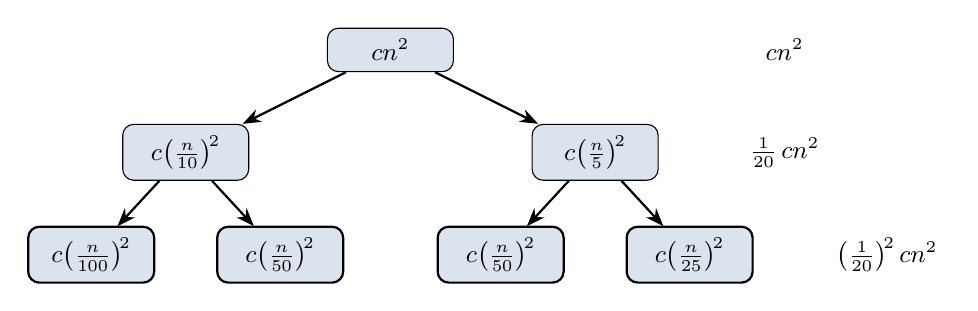
\begin{tikzpicture}[
    level distance=1.3cm,
    level 1/.style={sibling distance=5.2cm},
    level 2/.style={sibling distance=2.4cm},
    every node/.style={draw, rounded corners, fill=mLightBlue!20,
                        font=\small, inner sep=4pt, minimum width=1.6cm},
    edge from parent/.style={draw, -{Stealth}, thick},
    ann/.style={draw=none, fill=none, font=\small, anchor=west},
  ]
    \node {$cn^2$}
      child { node {$c\!\left(\tfrac{n}{10}\right)^{\!2}$}
        child { node {$c\!\left(\tfrac{n}{100}\right)^{\!2}$} }
        child { node {$c\!\left(\tfrac{n}{50}\right)^{\!2}$} }
      }
      child { node {$c\!\left(\tfrac{n}{5}\right)^{\!2}$}
        child { node {$c\!\left(\tfrac{n}{50}\right)^{\!2}$} }
        child { node {$c\!\left(\tfrac{n}{25}\right)^{\!2}$} }
      };
    \node[ann] at (4.2,  0.0) {$cn^2$};
    \node[ann] at (4.2, -1.3) {$\tfrac{1}{20}\,cn^2$};
    \node[ann] at (5.5, -2.6) {$\left(\tfrac{1}{20}\right)^{\!2} cn^2$};
  \end{tikzpicture}
  \end{center}

  \bigskip
  \begin{center}
    Each level costs $\dfrac{1}{20}$ of the level above $\;\Rightarrow\;$ geometric shrinkage.
  \end{center}
\end{frame}

\begin{frame}{Case 2: The Geometric Series}
  For $r < 1$:
  \[
    \sum_{i=0}^{\infty} r^i = \frac{1}{1-r},
    \qquad\text{e.g.}\qquad
    1 + \tfrac12 + \tfrac14 + \tfrac18 + \cdots = 2.
  \]

  \bigskip
  \begin{center}
  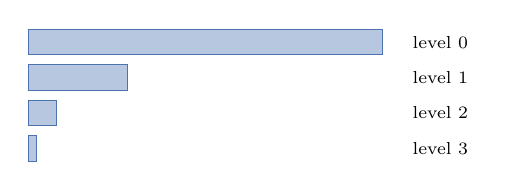
\begin{tikzpicture}[scale=0.9, every node/.style={transform shape}]
    \foreach \w [count=\i from 0] in {5.0, 1.4, 0.4, 0.12} {
      \fill[mLightBlue!40, draw=mLightBlue] (0,-\i*0.5) rectangle ++(\w,0.36);
      \node[right] at (5.3,-\i*0.5+0.18) {\scriptsize level \i};
    }
  \end{tikzpicture}
  \end{center}

  \bigskip
  \begin{center}
    The \alert{root} dominates: the total is a constant times the top level.
  \end{center}
\end{frame}

% ---------------------------------------------------------------- case 3
\begin{frame}{Case 3: Work Grows Geometrically}
  $T(n) = 7T(n/2) + cn^2$ \quad (Strassen's algorithm, later)

  \bigskip
  \begin{itemize}
    \item Level 0: \quad $cn^2$
    \item Level 1: \quad $7c\left(\frac{n}{2}\right)^2 = \frac{7}{4}cn^2$
    \item Level 2: \quad $7^2 c\left(\frac{n}{4}\right)^2 = \left(\frac{7}{4}\right)^2 cn^2$
  \end{itemize}

  \bigskip
  \begin{center}
  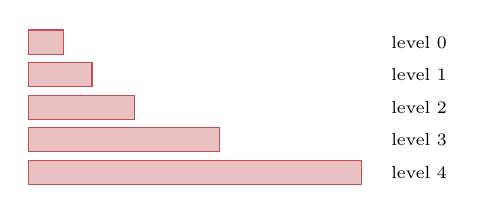
\begin{tikzpicture}[scale=0.9, every node/.style={transform shape}]
    \foreach \w [count=\i from 0] in {0.5, 0.9, 1.5, 2.7, 4.7} {
      \fill[mRed!35, draw=mRed] (0,-\i*0.46) rectangle ++(\w,0.34);
      \node[right] at (5.0,-\i*0.46+0.17) {\scriptsize level \i};
    }
  \end{tikzpicture}
  \end{center}

  \bigskip
  \begin{center}
    Now the \alert{deepest} level dominates.
  \end{center}
\end{frame}

\begin{frame}{Case 3: Recursion Tree}
  $T(n) = 7T(n/2) + cn^2$

  \begin{center}
  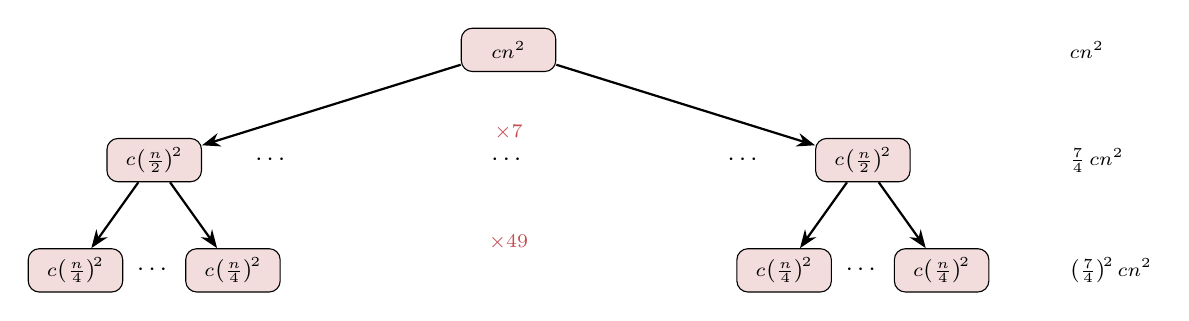
\begin{tikzpicture}[
    box/.style={draw, rounded corners, fill=mRed!20, font=\scriptsize,
                inner sep=3pt, minimum width=1.2cm, minimum height=0.55cm},
    dots/.style={font=\small, inner sep=2pt},
  ]
    % level 0
    \node[box] (r) at (0, 0) {$cn^2$};

    % level 1: 7 children
    \node[box] (l1a) at (-4.5, -1.4) {$c\!\left(\tfrac{n}{2}\right)^{\!2}$};
    \node[dots]       at (-3.0, -1.4) {$\cdots$};
    \node[dots]       at ( 0.0, -1.4) {$\cdots$};
    \node[dots]       at ( 3.0, -1.4) {$\cdots$};
    \node[box] (l1b) at ( 4.5, -1.4) {$c\!\left(\tfrac{n}{2}\right)^{\!2}$};
    \node[font=\scriptsize, mRed] at (0,-1.05) {$\times 7$};

    % level 2: children of l1a
    \node[box] (l2a1) at (-5.5, -2.8) {$c\!\left(\tfrac{n}{4}\right)^{\!2}$};
    \node[dots]        at (-4.5, -2.8) {$\cdots$};
    \node[box] (l2a2) at (-3.5, -2.8) {$c\!\left(\tfrac{n}{4}\right)^{\!2}$};
    % level 2: children of l1b
    \node[box] (l2b1) at ( 3.5, -2.8) {$c\!\left(\tfrac{n}{4}\right)^{\!2}$};
    \node[dots]        at ( 4.5, -2.8) {$\cdots$};
    \node[box] (l2b2) at ( 5.5, -2.8) {$c\!\left(\tfrac{n}{4}\right)^{\!2}$};
    \node[font=\scriptsize, mRed] at (0,-2.45) {$\times 49$};

    % edges
    \draw[-{Stealth},thick] (r) -- (l1a);
    \draw[-{Stealth},thick] (r) -- (l1b);
    \draw[-{Stealth},thick] (l1a) -- (l2a1);
    \draw[-{Stealth},thick] (l1a) -- (l2a2);
    \draw[-{Stealth},thick] (l1b) -- (l2b1);
    \draw[-{Stealth},thick] (l1b) -- (l2b2);
    % work per level
    \node[draw=none, fill=none, font=\scriptsize, anchor=west] at (7.0,  0.0) {$cn^2$};
    \node[draw=none, fill=none, font=\scriptsize, anchor=west] at (7.0, -1.4) {$\tfrac{7}{4}\,cn^2$};
    \node[draw=none, fill=none, font=\scriptsize, anchor=west] at (7.0, -2.8) {$\left(\tfrac{7}{4}\right)^{\!2} cn^2$};
  \end{tikzpicture}
  \end{center}

  \begin{center}
    Level $i$ costs $\left(\dfrac{7}{4}\right)^{\!i} cn^2$ $\;\Rightarrow\;$ growing geometrically.
  \end{center}
\end{frame}

\begin{frame}{Case 3: Summing Up}
  With at most $\log_2 n$ levels,
  \[
    \begin{aligned}
      \sum_{i=0}^{\log_2 n} \left(\tfrac{7}{4}\right)^i cn^2
      &= c \cdot \frac{\left(\frac74\right)^{\log_2 n + 1} - 1}{\frac74 - 1}\, n^2 \\[0.4em]
      &= \Theta\!\left(n^2 \left(\tfrac74\right)^{\log_2 n}\right)
       = \Theta\!\left(n^2 \cdot n^{\log_2 (7/4)}\right).
    \end{aligned}
  \]

  \bigskip
  Since $2 + \log_2(7/4) \approx 2.807$:
  \begin{alertblock}{}
    \[ T(n) = O\!\left(n^{2.807\ldots}\right) \]
  \end{alertblock}
\end{frame}

% ---------------------------------------------------------------- master
\begin{frame}{Master Theorem}
  \begin{block}{}
    If $\;T(n) = a\,T(n/b) + O(n^d)$, then
    \[
      T(n) = \begin{cases}
        O(n^d)          & \text{if } d > \log_b a, \\
        O(n^d \log n)   & \text{if } d = \log_b a, \\
        O(n^{\log_b a}) & \text{if } d < \log_b a.
      \end{cases}
    \]
  \end{block}

  \bigskip
  \begin{center}
    The proof is a formalization of the three recursion-tree cases.
  \end{center}
\end{frame}

\begin{frame}{Exercise}
  Solve each recurrence with the Master theorem.

  \bigskip
  \begin{itemize}
    \item Binary search: \quad $T(n) = T(n/2) + O(1)$
    \bigskip
    \item Merge sort: \quad $T(n) = 2T(n/2) + O(n)$
    \bigskip
    \item Strassen: \quad $T(n) = 7T(n/2) + O(n^2)$
  \end{itemize}
\end{frame}

\begin{frame}{Solution}
  \begin{center}
  \begin{tabular}{lcccl}
    \toprule
    & $a$ & $b$ & $d$ & result \\
    \midrule
    Binary search & $1$ & $2$ & $0$ & $d = \log_2 1 = 0 \;\Rightarrow\; O(\log n)$ \\
    Merge sort    & $2$ & $2$ & $1$ & $d = \log_2 2 = 1 \;\Rightarrow\; O(n \log n)$ \\
    Strassen      & $7$ & $2$ & $2$ & $d < \log_2 7 \approx 2.81 \;\Rightarrow\; O(n^{\log_2 7})$ \\
    \bottomrule
  \end{tabular}
  \end{center}

  \bigskip
  \begin{center}
    \small The first two are the $d = \log_b a$ case; Strassen is the leaf-dominated case.
  \end{center}
\end{frame}

\begin{frame}{When It Does Not Apply}
  The Master theorem needs the exact form $a\,T(n/b) + O(n^d)$.

  \bigskip
  It says nothing about
  \[
    T(n) = T(n/10) + T(n/5) + O(n^2),
  \]
  because the two sub-problems have \alert{different sizes}.

  \bigskip
  \begin{center}
    For those, fall back on the recursion tree.
  \end{center}
\end{frame}

% ---------------------------------------------------------------- others
\begin{frame}{Example: $T(n) = T(\sqrt{n}) + O(1)$}
  \begin{center}
  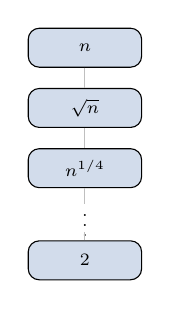
\begin{tikzpicture}[scale=0.9, every node/.style={transform shape},
      lv/.style={draw, rounded corners, fill=mLightBlue!25, minimum width=16mm, minimum height=5.5mm, inner sep=1pt}]
    \node[lv] (a) at (0,0)    {\scriptsize $n$};
    \node[lv] (b) at (0,-0.85) {\scriptsize $\sqrt{n}$};
    \node[lv] (c) at (0,-1.7)  {\scriptsize $n^{1/4}$};
    \node       at (0,-2.4)  {\scriptsize $\vdots$};
    \node[lv] (e) at (0,-3.0)  {\scriptsize $2$};
    \draw[mGray] (a) -- (b); \draw[mGray] (b) -- (c); \draw[mGray] (c) -- (0,-2.2);
    \draw[mGray] (0,-2.6) -- (e);
  \end{tikzpicture}
  \end{center}

  Each level does $O(1)$ work, so we just count levels $k$:
  \[
    n^{1/2^k} = 2
    \;\Longrightarrow\;
    \frac{1}{2^k}\log_2 n = 1
    \;\Longrightarrow\;
    k = \log_2(\log_2 n).
  \]

  \begin{center}
    Hence $T(n) = O(\log \log n)$.
  \end{center}
\end{frame}

\begin{frame}{Example: $T(n) = T(n-1) + O(n^2)$}
  The tree is a \alert{path} of length $n$: \; $n \to n-1 \to n-2 \to \cdots \to 1$.

  \bigskip
  Level $i$ does $c(n-i)^2$ work, so
  \[
    T(n) = c\left(n^2 + (n-1)^2 + \ldots + 1^2\right) = \Theta(n^3),
  \]
  using $1^c + 2^c + \ldots + n^c = \Theta(n^{c+1})$ from the previous chapter.

  \bigskip
  \begin{center}
    \small Shrinking by a constant \emph{amount} is very different from shrinking by a constant \emph{factor}.
  \end{center}
\end{frame}



\end{document}
